\section*{Introduction}
\addcontentsline{toc}{section}{Introduction}

In a discussion of hypercubes of all dimensions \cite{gardner1977}, Martin
Gardner posed the problem of finding the largest square which fits into a unit
cube (i.e., a cube of unit side), as well as the largest cube in a unit
tesseract.  He gave the solution to the largest square in a cube, but he stated
that the problem of the largest cube in a tesseract was still unsolved. Seven
people had sent him solutions, all different, and since none of these proofs
had been published or checked by mathematicians, he regarded the problem
as still unsolved. Even in a later edition of his book \cite{gardner1989},
Gardner wrote that nothing had been published on the problem.

Soon after I started thinking about these problems, I started
wondering about the largest square in a tesseract. This led me to
generalize the problem to finding the largest m-cube (that is, an mdimensional
cube) in an n-cube, for all m and n for which the problem
makes sense: $1 \leq m \leq n$.

I found the solution for all $(m,n)$ where $m$ divides $n$, and also for all
n when $m = 2$. I have a candidate for $(m,n) = (3,4)$, but I have not yet been
able to prove that it is the largest cube in a tesseract\footnote{Yes, I have,
see Appendix A}.  Letting $f(m,n)$ denote the side of the largest m-cube in
an n-cube of unit side, I have a lower bound for $f(3,4)$. I have proved
several inequalities involving $f(m,n)$, and I have done additional work on
$m = 3$, $n = 4$, and for $n = m + 1$, in general.

\section*{Method of Solution}
\addcontentsline{toc}{section}{Method of Solution}

instead of thinking about the largest m-cube in an n-cube, we will
consider a unit m-cube in an arbitrary orientation in Euclidean n-space,
and try to find the smallest n-cube that contains the m-cube, where the n-cube
is in a ``standard orientation'': i.e., all of its edges are parallel to
Cartesian coordinate axes.

We may assume that one of the vertices of the m-cube is at the
point $\vec{P}_0$ , and that the $m$ orthonormal vectors in n-space,
$\vec{v}_i$, $i = 1, 2, \cdots, m$
are such that the $2m$ vertices of the m-cube are at
$\vec{P}_0, \vec{P}_0+\vec{v}_1, \vec{P}_0+\vec{v}_2, \cdots, \vec{P}_0+\vec{v}_m,
\vec{P}_0+\vec{v}_1+\vec{v}_2, \cdots,
\vec{P}_0+\vec{v}_1+\vec{v}_2+\cdots+\vec{v}_m$. 
We need to determine how far the m-cube extends in each of the n coordinate
directions. Since the m-cube is the convex hull of its vertices, we need only
consider the vertices. We let $v_{ij}$ represent the $j$th component of $v_i$,
$j$ = 1 through $n$. A little thought leads to the conclusion that $R_j$, the
range in the jth direction in n-space, is given by
\begin{equation*}
R_j = \sum_{i=1}^{n} | v_{ij} |
\end{equation*}
Then the smallest n-cube in a standard orientation which contains the m-cube
has a side equal to
\begin{equation*}
R = \max_{j=1}^{n} R_j.
\end{equation*}
Thus we want to minimize $R$, where
\begin{equation*}
R = \max_{j=1}^{n} \left( \sum_{i=1}^{m} | v_{ij} | \right),
\end{equation*}
where
\begin{equation*}
\sum_{k=1}^{n} v_{ik} v_{jk} = \delta_{ij}
\end{equation*}
where $\delta_{ij} = 1$ for $i = j$, and $0$ otherwise.

Then $f(m,n)$ is the reciprocal of the minimum value of $R$. We know that $R$
really has a minimum and not just an infimum, because $R$ is a continuous
function of the $v_{ij}$, and the $v_{ij}$ satisfying the above equation form
a compact set in an mn-dimensional Euclidean space.

If all of the $R_i$ are equal, then we call the m-cube ``snug-fitting'' --
it fits snugly into the n-cube in the sense that it cannot undergo any
translation and remain within the n-cube.

In some of our calculations, we will find it convenient to use a
different normalization, such that the n-cube does have unit side,
instead of the m-cube; thus, all the $\vec{v}_i$ will still have equal
lengths but they will (usually) not have unit length.

We will describe embeddings of m-cubes in n-cubes by m x n
matrices such that each row of a matrix represents the components of
one of the $\vec{v}_i$. Thus the matrix element in the $i$th row and the $j$th
column will be $v_{ij}$. The rows of the matrix will be mutually perpendicular
and have equal lengths as vectors. We want to minimize the maximum of the
``column-sums'' (the sum of the absolute values of the numbers in each
column) while keeping the row vectors mutually perpendicular and leaving
their lengths unchanged.

These $v_{ij}$ matrices, which we shall also call $V$ matrices, have the
property that the lengths of the row vectors, the maximum range, and the
orthogonality of the rows are unaffected by certain trivial
transformations: the interchange of any two rows or columns, and the
multiplication of the elements of any row or column by -1.

\section*{When does $f(m,n) = \sqrt{n/m}$?}
\addcontentsline{toc}{section}{When does $f(m,n) = \sqrt{n/m}$?}

For $m = 1$, an m-cube is a line segment. The longest line segment in
an n-cube of unit side is the main diagonal, so $f(1,n) = \sqrt{n}$. If an
m-cube is inscribed in an n-cube, then the longest line segment in the m-cube
cannot be longer than the longest line segment in the n-cube, so that
$f(m,n) \leq \sqrt{n/m}$. When does equality occur, besides $m = 1$?

Assume $m \geq 2$. For $f(m,n) = \sqrt{n/m}$, each main diagonal of the m-cube
must be a main diagonal of the n-cube. Thus,
\begin{equation*}
\pm \vec{v}_1 \pm \vec{v}_2 \pm \cdots \pm \vec{v}_m = (\pm 1, \pm 1, \cdots, \pm 1)
\end{equation*}
for all combinations of + and - signs on the left-hand side. Now, change
the sign in front of one of the $vec{v}_i$, and subtract and divide by 2. Then
\begin{equation*}
\vec{v}_i = (\text{combination of 1's, -1's, and 0's})
\end{equation*}
Since all of the $\vec{v}_i$ have length $\sqrt{n/m}$, there are $(n/m) \pm 1$'s
among the components of each of the $\vec{v}_i$. Thus $n/m$ must be an integer.
Each row of the matrix of $\vec{v}_i$ components has $(n/m) \pm 1$'s and the
rest zeros.

The $V$ matrix has $m$ rows and $n$ columns, so the entire matrix
contains $n \pm 1$'s. There cannot be a column of all zeros, so each column
contains exactly one $\pm 1$.• By making trivial transformations, we can
transform the matrix into $n/m$ copies of the m x m identity matrix placed
side by side. Thus equality occurs if and only if $m$ divides $n$, and the
maximal m-cubes are unique up to trivial transformations. These maximal
m-cubes are snug-fitting, and they have the property that all of the
vertices of the m-cube are also vertices of the n-cube.

The $V$ matrix for the largest square in a tesseract, for example, may
be written as
\begin{equation*}
\begin{bmatrix}
1 & 0 & 1 & 0 \\
0 & 1 & 0 & 1
\end{bmatrix}
\end{equation*}
or as
\begin{equation*}
\begin{bmatrix}
1 & 1 & 0 & 0 \\
0 & 0 & 1 & 1
\end{bmatrix}
\end{equation*}
A projection of it is shown in Figure~\ref{fig1}.
\begin{figure}
\begin{center}
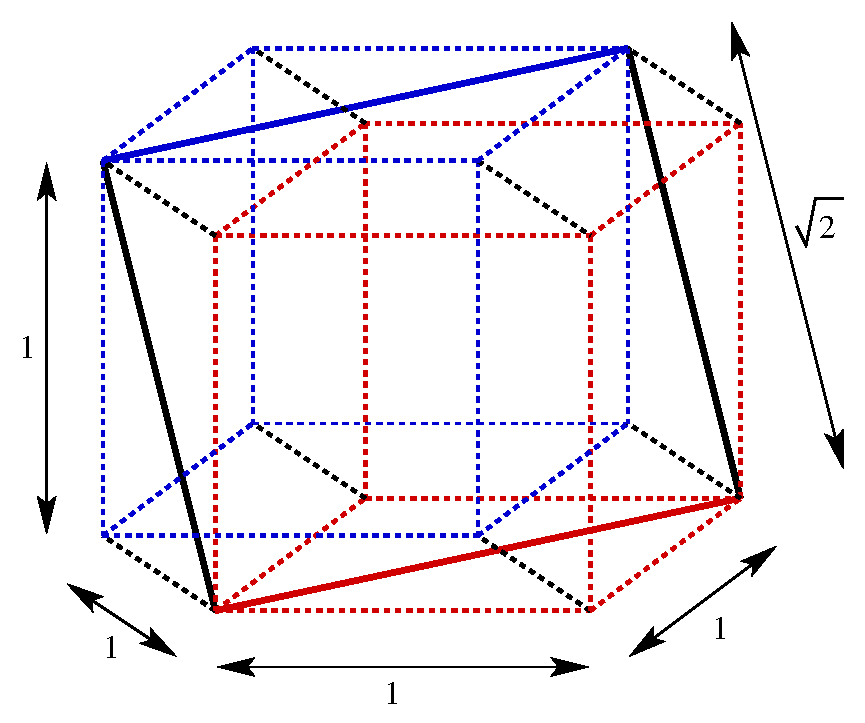
\epsfig{file=figure1.eps,width=4.5in}
\end{center}
\vspace{-0.2in}
\caption{The largest square in a tesseract.}
\label{fig1}
\end{figure}
The largest 4-cube in a, 2-cube may be written as
\begin{equation*}
\begin{bmatrix}
1 & 1 & 1 & 0 & 0 & 0 & 0 & 0 & 0 & 0 & 0 & 0 \\
0 & 0 & 0 & 1 & 1 & 1 & 0 & 0 & 0 & 0 & 0 & 0 \\
0 & 0 & 0 & 0 & 0 & 0 & 1 & 1 & 1 & 0 & 0 & 0 \\
0 & 0 & 0 & 0 & 0 & 0 & 0 & 0 & 0 & 1 & 1 & 1
\end{bmatrix}
\end{equation*}

\section*{Looking for the Largest Cube in a Tesseract}
\addcontentsline{toc}{section}{Looking for the Largest Cube in a Tesseract}

To try to find the largest cube in a tesseract, I computed formulas for the
components of three orthonormal vectors $\vec{v}_i$, in 4-space, which were
functions of 6 angles (similar to the 3 Euler angles used to specify the
orientation of a rigid body in 3-space). For each orientation (with the
angles varying in steps of $5^o$), the computer computed R. and we printed
the cases in which $R < 1$. The results suggested that the smallest value of
$R$ occurs when the cube is snug-fitting ($R_1$ = $R_2$ = $R_3$ = $R_4$) and
the $V$ matrix has a triangle of zeros:
\begin{equation*}
\begin{bmatrix}
A & B & 0 & 0 \\
F & G & H & 0 \\
K & L & M & P
\end{bmatrix}
\end{equation*}
We shall prove that, of all matrices with orthonormal rows and zeros as
above, the minimum value of $R$ occurs when all ``column-sums'' are equal,
and we find this value of $R$.

The above matrix can be parameterized in terms of 3 angles (where
\label{refpage4}
$s_\alpha = sin~\alpha, c_\alpha = cos~\alpha$, etc.):
\begin{equation*}
\begin{bmatrix}
-s_\alpha                  & -c_\alpha                  &  0                & 0        \\
-c_\alpha s_\beta          &  s_\alpha s_\beta          & -c_\beta &        0          \\
-c_\alpha c_\beta s_\gamma &  s_\alpha c_\beta s_\gamma &  s_\beta s_\gamma & -c_\gamma
\end{bmatrix}
\end{equation*}
We want to find the values of $\alpha$, $\beta$, and $\gamma$ which
minimize $R$.

From the above matrix,
\begin{equation*}
R_1 = | s_\alpha | + | c_\alpha s_\beta | + | c_\alpha c_\beta s_\gamma |, etc.
\end{equation*}
If we let $\alpha'$ be the angle (in the first quadrant) such that
$sin~\alpha' = | sin~\alpha |$, $cos~\alpha' = | cos~\alpha |$, and
similarly for $\beta$ and $\gamma$, then we may write
\begin{align*}
R_1 & = s_{\alpha'} + c_{\alpha'} s_{\beta'} + c_{\alpha'} c_{\beta'} s_{\gamma'} \\
R_2 & = c_{\alpha'} + s_{\alpha'} s_{\beta'} + s_{\alpha'} c_{\beta'} s_{\gamma'} \\
R_3 & = c_{\beta'} + s_{\beta'} s_{\gamma'} \\
R_4 & = c_{\gamma'}
\end{align*}
with $0 \leq \alpha',\beta',\gamma' \leq 90^o$.

Since $R = \max_{i=1}^{4} R_i$ is a continuous function of $\alpha'$,
\label{refpage3}
$\beta'$, and $\gamma'$ on a compact set, there must be a minimum value.
We can prove that this minimum value is strictly less than 1, by showing
\label{refpage29}
that we can choose the angles so that $R$ is less than 1.

First, choose $\alpha'$ so that $0^o < \alpha' < 90^o$ . Then $sin\alpha'$
and $cos\alpha'$ are less than 1.  Next, choose $\beta'$ such that
$s_{\alpha'} + c_{\alpha'} s_{\beta'}$ and
$c_{\alpha'} + s_{\alpha'} s_{\beta'}$ and
$c_{\beta}'$ are less than 1. Finally, choose $\gamma'$ so that
$R_1$ $R_2$, $R_3$, and $R_4$ are all less than 1.

We will now prove that the minimum of $R$ occurs at values of $\alpha'$,
$\beta'$, and $\gamma'$ which make all of the $R_i$ equal.

First we show that the minimum does not occur on the boundary
(where at least one of $\alpha'$, $\beta'$, $\gamma'$
is $0^o$ or $90^o$).  If $\alpha' = 0$, then $c_{\alpha'} = 1$ so
that $R_2 \geq 1$. Similarly, if $\beta' = 0$, then $R_3 \geq 1$, and
if $\gamma' = 0$, then $R_4 \geq 1$.

If $\alpha' = 90^o$, then $c_{\alpha'} = 0$ so we have zeros at least in the
following places:
\begin{equation*}
\begin{matrix}
X & 0 & 0 & 0 \\
0 & X & X & 0 \\
0 & X & X & X
\end{matrix}
\end{equation*}
Then in the upper left corner we must have a 1, so $R \geq 1$. If
$\beta' = 90^o$, then $cos\beta' = 0$, so we have
\begin{equation*}
\begin{matrix}
X & X & 0 & 0 \\
X & X & 0 & 0 \\
0 & 0 & X & X
\end{matrix}
\end{equation*}
The upper left 2 x 2 matrix now corresponds to the largest square in a
square, so that $max(R_1,R_2) \geq 1$ so $R \geq 1$. Finally, if
$\gamma' = 90^o$ then we have $cos\gamma' = 0$, so the matrix looks like
this:
\begin{equation*}
\begin{matrix}
X & X & 0 & 0 \\
X & X & X & 0 \\
X & X & X & 0
\end{matrix}
\end{equation*}
and now we have the largest cube in a cube, so $max(R_1,R_2,R_3) \geq 1$,
so $R \geq 1$. Thus the minimum does not occur on the boundary, so we can now
assume that $0^o < \alpha', \beta', \gamma' < 90^o$.

Suppose $R = R_1 > R_2, R_3, R_4$ - we say that the only ``maximal column'' is
the first column.  Then we can decrease $R_1$ slightly by decreasing $\gamma'$.
This decreases $R$.

Similarly, if $R = R_2$ and the only maximal column is column 2, then
we decrease $\gamma'$, thus decreasing $R$.  This also works if the maximal
column is column 3, or even if there are 2 or 3 maximal columns among the
first three columns.

If instead $R_4$ is the largest, we increase $\gamma'$ slightly, which
decreases $R$.  Next, suppose $R_1$ and $R_4$ are largest.  Note that
$\partial^2 R_1 / \partial {\alpha'}^2 < 0$, while $R_4$ is independent of
$\alpha'$.  Thus, if $\partial R_1  / \partial \alpha' > 0$, we decrease
$\alpha'$ slightly, decreasing $R_1$ and leaving $R_4$ unchanged.  If
$\partial R_1  / \partial \alpha' < 0$, we increase $\alpha'$ to decrease
$R_1$.  If $\partial R_1  / \partial \alpha'$ happens to be zero, then since
the second derivative is negative we can decrease $R_1$ by changing $\alpha'$
slightly in either direction.  This reduces this case to the case in which
only $R_4$ is equal to $R$ since we could have changed $\beta'$ instead.

If $R_2$ and $R_4$ are largest, a similar argument applies.  If $R_3$ and
$R_4$ are largest, a similar argument shows that we can decrease $R_3$ by
changing $\beta'$ slightly.

If $R_1$, $R_3$, and $R_4$ or $R_2$, $R_3$, and $R_4$ are largest, then we
change $\alpha'$ slightly, reducing it to the case in which only $R_3$ an
$R_4$ are largest.

The last case to consider is the one where $R_1$, $R_2$, and $R_4$ are
largest.  Since $R_1 = R_2$,
\begin{equation*}
(s_{\alpha'})(1 - s_{\beta'} - c_{\beta'} s_{\gamma'}) =
(c_{\alpha'})(1 - s_{\beta'} - c_{\beta'} s_{\gamma'})
\end{equation*}
Thus, either $\alpha' = 45^o$ or $s_{\beta'} + c_{\beta'} s_{\gamma'} = 1$ or
both.

If $\alpha' = 45^o$, then we can change $\beta'$ slightly so that $R_1$ and
$R_2$ both decrease while $R_4$ is unchanged.

If $s_{\beta'} + c_{\beta'} s_{\gamma'} = 1$, then $R_1 = sin\alpha' +
cos\alpha'$, but then $R_1 \geq 1$, so this is not a maximal cube.  Also,
$R_1$ cannot be equal to $cos\gamma'$.

We have thus found that the minimum $R$ occurs when $\alpha'$, $\beta'$, and
$\gamma'$ are chosen such that $R_1 = R_2 = R_3 = R_4 = R$.  This will give us
the largest cube in a tesseract with a triangle of three zeros in its $V$
matrix.  The three equations in $\alpha'$, $\beta'$, and $\gamma'$, with
$cos\gamma' = R$, can be reduced to an equation for $R$ alone after doing a
lot of algebra:
\begin{equation*}
4 R^4 - 6 \sqrt{2} R^3 + 11 R^2 - 6 \sqrt{2} R + 2 = 0
\end{equation*}
We can get rid of the square roots, which occur because $\alpha' = 45^o$, and
we obtain
\begin{equation*}
16 R^8 + 16 R^6 - 7 R^4 - 28 R^2 + 4 = 0
\end{equation*}
Finally, letting $x = 1/R^2$, we get
\begin{equation*}
4 x^4 - 28 x^3 - 7 x^2 + 16 x + 16 = 0
\end{equation*}
There may be extraneous roots, but we know that at least one root is genuine
because of our previous work and corresponds to the largest cube in a tesseract
with the triangle of zeros in its $V$ matrix.

Using the quartic equation formula, we find that there is only one root in the
appropriate range that is between 1 and 4/3; we call this root $x_0$.  The
side of this cube in a unit tesseract is $\sqrt{x_0}$, where
\begin{equation*}
x_0 = 7/4 + r/2 - d/2
\end{equation*}
where
\begin{align*}
d & = \sqrt{105/4 - y + 90/r}                 \\
r & = \sqrt{14+y}                             \\
y & = a + b - 7/12                            \\
a & = \sqrt[3]{184841/1728 + 5 \sqrt{1290}/2} \\
b & = \sqrt[3]{184841/1728 - 5 \sqrt{1290}/2}
\end{align*}
These formulas yield $\sqrt{x_0} \approx 1.00743475688$.

Thus, we now have a rigorous proof that $f(3,4) \geq \sqrt{x_0}$ where $x_0$
is the root of $4 x^4 - 28 x^3 - 7 x^2 + 16 x + 16 = 0$ which is between 1 and
4/3.

\section*{Other cases where $n = m+1$}
\addcontentsline{toc}{section}{Other cases where $n = m+1$}

Similar arguments apply when $m$ = 1, 2, 4, and 5; the number of angles is
equal to m.  The matrices have the forms
\begin{equation*}
\begin{array}{rclc}

\left[
\begin{array}{cc}
-s_\alpha & -c_\alpha
\end{array}
\right]
&
\rightarrow
&
\left[
\begin{array}{cc}
-\sqrt{2}/2 & -\sqrt{2}/2
\end{array}
\right]
& (m = 1) \\

& & & \\

\left[
\begin{array}{ccc}
-s_\alpha         & -c_\alpha         & 0       \\
-c_\alpha s_\beta & -s_\alpha s_\beta & c_\beta \\
\end{array}
\right]
&
\rightarrow
&
\left[
\begin{array}{rrc}
-\sqrt{2}/2 & -\sqrt{2}/2 &  0            \\
-\sqrt{2}/6 &  \sqrt{2}/6 & -2 \sqrt{2}/3 \\
\end{array}
\right]
& (m = 2)

\end{array}
\end{equation*}
or with a different normalization:
\begin{equation*}
\begin{array}{ll}

\left[
\begin{array}{rr}
1/2 & 1/2
\end{array}
\right]
& (m=1) \\

& \\

\left[
\begin{array}{rrr}
3/4 &  3/4 & 0 \\
1/4 & -1/4 & 1 \\
\end{array}
\right]
& (m=2)

\end{array}
\end{equation*}
For $m = 4$, the triangle of zeros looks like this:
\begin{equation*}
\begin{bmatrix}
X & X & 0 & 0 & 0 \\
X & X & X & 0 & 0 \\
X & X & X & X & 0 \\
X & X & X & X & X
\end{bmatrix}
\end{equation*}
while for $m = 5$, we have:
\begin{equation*}
\begin{bmatrix}
X & X & 0 & 0 & 0 & 0 \\
X & X & X & 0 & 0 & 0 \\
X & X & X & X & 0 & 0 \\
X & X & X & X & X & 0 \\
X & X & X & X & X & X
\end{bmatrix}
\end{equation*}
In the next section we will give a procedure for computing the sines and
cosines of the matrix elements for all $m$.

Although I have not given a rigorous inductive proof, it seems clear that
$f(m,m+1)$ is always strictly greater than 1.  For $m = 2$, we obtain Martin
Gardner's square in a cube.  However, we have not yet proved that it is
optimal.

By considering these matrices for $n = m+1$, with the triangles of zeros and
the parameterizations in terms of sines and cosines of $m$ angles, we can
derive a lower bound for $f(m,m+1)$ which is larger than 1.  We shall not
describe the proof here, but the result is that, for $m > 1$:
\begin{equation*}
f(m,m+1) > \frac{1}{1-[(1-\sqrt{2}/2)^{3^{m-1}}/32^{(3^{m-1}-1)/2}]}
\end{equation*}
\label{refpage28}
In deriving this lower bound, I actually used a formula from special
relativity!  I needed a ``nice'' function of two variables to use in place of
the ``max'' function.  Both variables were less than 1 and I wanted the
function to be less than 1 and, at least, as large as both of them.  So I used
the velocity addition formula from special relativity with ``c'', the velocity
of light, set equal to 1!

\section*{Plane (2-dimensional) rotations}
\addcontentsline{toc}{section}{Plane (2-dimensional) rotations}

For any $V$ matrix, we can obtain a new one by a rotation involving two
columns, where column $i$ becomes $(\text{column}~i)\allowbreak~cos\theta +
(\text{column}~j)\allowbreak~sin\theta$ and column $j$ becomes $(\text{column}~j)
cos\theta - (\text{column}~i)\allowbreak~sin\theta$.  In fact, the matrices in
the previous section can be obtained by starting with a matrix such as
\begin{equation*}
\begin{array}{cc}

\begin{bmatrix}
1 & 0 & 0 & 0 \\
0 & 1 & 0 & 0 \\
0 & 0 & 1 & 0
\end{bmatrix}
& (m = 3) \\

& \\

\begin{bmatrix}
1 & 0 & 0 & 0 & 0 \\
0 & 1 & 0 & 0 & 0 \\
0 & 0 & 1 & 0 & 0 \\
0 & 0 & 0 & 1 & 0
\end{bmatrix}
& (m = 4)

\end{array}
\end{equation*}
and performing $m$ rotations through different angles, in which the $i$th
rotation involves columns $i$ and $m+1$.

\section*{Using small rotations to decrease $R_i$ (or ``column-sums'')}
\addcontentsline{toc}{section}{Using small rotations to decrease $R_i$ (or ``column-sums'')}

In this section we shall prove two useful theorems, although we will discuss
specific cases to make the proofs less abstract and easier to understand.

Suppose that $(A, B, C)^\top$ and $(D, E, F)^\top$ are the $i$th and $j$th columns,
respectively, of a $V$ matrix.  Let $a =$ sign of $A$, $b =$ sign of $B$, etc.
Assume that the $i$th column contains no zeros.  Let us make a rotation:
$\text{column}~i \rightarrow (\text{column}~i)\allowbreak~cos\theta +
(\text{column}~j)\allowbreak~sin\theta$, $\text{column}~j \rightarrow
(\text{column}~j)\allowbreak~cos\theta - (\text{column}~i)\allowbreak~sin\theta$. Then,
$A \rightarrow A~cos\theta + D~sin\theta$, so that $|A| \rightarrow | A~
cos\theta + D~sin\theta | = a (A~cos\theta + D~sin\theta$ if $\theta$
sufficiently near zero.  We find that $d|A|/d\theta$ at $\theta = 0$ is $aD$,
while $d^2|A|/d\theta^2$ at $\theta = 0$ is $-|A|$.  Thus, $dR_i/d\theta$ at
$\theta = 0$ is $a D + b E + c F$, while $d^2R_i/d\theta^2$ at $\theta = 0$ is
$-|A|-|B|-|C|$, which is always negative.

This shows that we can always decrease $R_i$ by making a small rotation.  This
theorem, which we shall call Theorem 1, can often be used to decrease R in
particular situations to show that a particular $V$ matrix is not optimal.
For instance, if a $V$ matrix with no zeros is not snug-fitting, then one can
make small rotations to decrease R, so the m-cube cannot be optimal.

Even if the $i$th column contains zeros, we may still decrease its column-sum
if the $j$th column contains a zero in every row in which the $i$th column
contains a zero (unless, of course, the $i$th column contains all zeros).

Theorem 1 can be used, in most places, instead of our arguments about
increasing or decreasing th angles $\alpha'$, $\beta'$, and $\gamma'$, to show
that we can decrease R for our cube in the tesseract.  One has to be careful
sometimes to perform the small rotations in a particular order, since rotating
columns $i$ and $j$ may change a zero in column $j$ to a nonzero number, which
may prevent some other rotation from decreasing $R$.

Another useful theorem about two columns is especially useful where $R_i =
R_j$, and shows that sometimes we can decrease $R_i$ and $R_j$ simultaneously.
Let the $i$th and $j$th columns be $(A, B, C)^\top$ and $(D, E, F)^\top$
as before.  Suppose that $A$, $B$, $C$, and $D$ are positive and $E$ and $F$
are negative.  Then $d R_i/d \theta$ at $\theta = 0$ is $a D + b E + c F$,
while $d R_j/d \theta$ at $\theta = 0$ is $-d A - e B - f C$.  So $d R_i/d
\theta$ at $\theta = 0$ is $D + E + F = D - |E| - |F|$ while $d R_j/d \theta$
at $\theta = 0$ is $- A + B + C$. Assuming that neither derivative is zero,
the two derivatives have the same sign if $A - B - C$ and $D - |E| - |F|$ have
opposite signs, then $R_i$ and $R_j$ can both be reduced by the same small
rotation.  We shall call the Theorem 2.

Both of these theorems will be used in the next section, in order to find the
largest square in an odd-dimensional cube.

\section*{The Largest Square in an Odd-Dimensional Cube}
\addcontentsline{toc}{section}{The Largest Square in an Odd-Dimensional Cube}
\label{refpage18}

To find the largest square in an n-dimensional cube for all odd $n$, we shall
find it convenient to distinguish two possibilities:
\begin{enumerate}
\item{$f(2,3) > 1$}
\item{$f(2,3) = 1$}
\end{enumerate}
We may already know that $f(2,3) > 1$, but we will pretend we don't know that,
to show that we can prove it and derive the largest square in any
odd-dimensional cube, without being clever enough to guess it first.

Consider possibility (1).  We normalize the $V$ matrix so that the largest
column-sum is 1.  If $f(2,3) > 1$, then we can append a 2x2 identity matrix to
the 2x3 $V$ matrix to obtain a valid $V$ matrix for $n = 5$, so that $f(2,5)^2
\geq f(2,3)^2 + 1$.  We can continue this process indefinitely, to show that
if $f(2,3) > 1$, then $f(2,5) > \sqrt{2}$, $f(2,7) > \sqrt{3}$ and so on.

We will first prove that, for maximality, all column-sums are equal.  That is,
the square is snug-fitting:  it touches all hyperfaces on the n-dimensional
cube.

First of all, the optimal $V$ matrix cannot have any columns which have both
entries equal to zero.  For if it had an all-zero column, the matrix would
correspond to the largest square in an (n-1)-cube, and we would be in
possibility (2).  Thus, each column of the $V$ matrix either has both entries
nonzero (we will call this type 1), or has a zero in the second row (type 2)
or in the first row (type 3), but not both.  The idea of the proof is to
attempt to use Theorem 1 to show that, for each of the three types of columns,
all the maximal columns can be ``shrunk'' (have their $R_i$ values decreased),
by performing small rotations with other columns of the same type.  So we have
to determine when this will not work.  If this procedure were always possible,
we would know already that the maximal square in any odd-dimensional cube must
be snug-fitting, if possibility (2) is correct.  Actually, columns with no
zeros can be made smaller by rotating them with any type column.  The only
difficulty occurs if there are maximal columns with a zero, with no
corresponding non-maximal columns to rotate them with.  We may assume that all
the columns with both elements nonzero have been shrunk and are non-maximal.
Thus, the matrix looks like this:
\begin{equation*}
\left[
\begin{array}{c|c|c}

\text{nonzero}             &
\text{nonzero (all equal)} &
0~0~\cdots~0               \\

\text{(all non-maximal)}   &
0~0~\cdots~0               &
\text{nonzero (all equal)}

\end{array}
\right]
\end{equation*}
Because the two rows of the matrix are orthogonal, the shorter rows of the
nonzero part are also orthogonal.  Then we can reduce the nonzero elements of
type 3 by some constant factor, and multiply the second row type 1 elements
by a common factor to increase them slightly, so that $\vec{v}_2$ remains the
same length.  We can do a similar thing for the type 2 columns.  This reduces
$R$.  This will work unless there are no type 1 columns; that is, every column
has a zero.  So we will show that such a $V$ matrix cannot be maximal.

If the maximum column-sum is normalized to 1, then for $n$ odd, since all
elements are $\leq 1$, then $f(2,n)^2$ is at most $(n-1)/2$.  But then we have
case (2), a contradiction.  This completes the proof that any optimal matrix
is snug-fitting.

We will also need to show that neither $\vec{v}_1 + \vec{v}_2$ nor $\vec{v}_1
- \vec{v}_2$ can have any zero components.  Either one of these would
represent a line segment in a unit (n-1)-cube, which is the diagonal of the
inscribed square.  To obtain the side of the square, we divide $\sqrt{n-1}$ by
$\sqrt{2}$.  Thus, $f(2,n)$ cannot be greater than $\sqrt{(n-1)/2}$, which is
possibility (2).

Therefore, the $V$ matrix can be written as
\begin{equation*}
\left[
\begin{array}{ccc|cc|ccc|ccc}

a_1   & a_2   & \cdots & b_1      & \cdots & 1 & \cdots & 1 & 0 & \cdots & 0 \\
1-a_1 & 1-a_2 & \cdots & -(1-b_1) & \cdots & 0 & \cdots & 0 & 1 & \cdots & 1

\end{array}
\right]
\end{equation*}
where none of the $a_i$ or $b_i$ are equal to $1/2$.

Next, we assume, with no loss of generality, that one of the $a_i$ is greater
than $1/2$.  Then, by Theorem 2, each of the $b_i$ must be greater than $1/2$;
otherwise we could reduce at least two column-sums.  Applying this theorem
again, we find that all of the $a_i$ must also be greater than $1/2$.  So we
can now write the matrix as
\begin{equation*}
\left[
\begin{array}{ccc|cc|ccc|ccc}

1/2 + c_1 & 1/2 + c_2 & \cdots & ~~1/2 + d_1  & \cdots & 1 & \cdots & 1 & 0 & \cdots & 0 \\
1/2 - c_1 & 1/2 - c_2 & \cdots & -(1/2 - d_1) & \cdots & 0 & \cdots & 0 & 1 & \cdots & 1

\end{array}
\right]
\end{equation*}
All the $c_i$ and $d_i$ are strictly between $0$ and $1/2$.  In the above
matrix we now have four possible types of columns, and the numbers of columns
of each type will be called $i_+$, $i_-$, $i_1$, and $i_0$, from left to right.

Now we can use the method of Lagrange multipliers to find possible maximal $V$
matrices.  There are two constraints:  the two rows of the matrix, $\vec{v}_1$
and $\vec{v}_2$, are orthogonal and have equal lengths.  We want to maximize,
say, $|\vec{v}_1|^2$.  The constraints are
\begin{equation*}
\sum_{i=1}^{i_+} (1/2 + c_i)(1/2 - c_i) -
\sum_{i=1}^{i_-} (1/2 + d_i)(1/2 - d_i) = 0
\end{equation*}
\begin{equation*}
\sum_{i=1}^{i_+} (1/2 + c_i)^2 +
\sum_{i=1}^{i_-} (1/2 + d_i)^2 + i_1 =
\sum_{i=1}^{i_+} (1/2 - c_i)^2 +
\sum_{i=1}^{i_-} (1/2 - d_i)^2 + i_0
\end{equation*}
where we wish to maximize
\begin{equation*}
\sum_{i=1}^{i_+} (1/2 + c_i)^2 + \sum_{i=1}^{i_-} (1/2 + d_i)^2 + i_1.
\end{equation*}
These equations simplify to:
\begin{equation*}
(1/4)(i_+ - i_-) - \sum_{i=1}^{i_+} c_i^2 + \sum_{i=1}^{i_-} d_i^2 = 0
\end{equation*}
\begin{equation*}
2 \sum_{i=1}^{i_+} c_i + 2 \sum_{i=1}^{i_+} d_i + i_1 - i_0 = 0
\end{equation*}
where we want to maximize
\begin{equation*}
\sum_{i=1}^{i_+} (c_i^2 + c_i) + \sum_{i=1}^{i_-} (d_i^2 + d_i) +
(1/4)(i_+ + i_-) + i_1.
\end{equation*}
However, there is a theorem which will tell us that none of the ``points'' we
find by using the Lagrange multipliers will be a maxima.  This is the second
derivative test for constrained relative maxima.  The proof of this theorem is
given as a homework exercise in \cite{fleming1965}.  This theorem is a
generalization of the second derivative test used when maximizing an
unconstrained function of several variables, to determine whether a particular
critical point is a maximum, a minimum, or a saddle point.  The unconstrained
theorem tells us to look at the matrix of second partial derivatives of the
function: if this matrix is negative definite, then the point is a local
maximum, and if the point is a local maximum then the matrix is negative
semidefinite.

In the constrained version of the theorem, the test is the same,
except that in place of the function to be maximized, we use this function
plus the sum of the Lagrange multipliers multiplied by the corresponding
constraints.

In our particular optimization problem, the variables are the $c_i$ and the
$d_i$, and there must be at least one $c_i$ and at least one $d_i$. This is
because, as we have already shown, we never obtain a maximal square in an
odd-dimensional cube when every column of the $V$ matrix contains a zero, and,
since the rows are orthogonal, the existence of a $c_i$ requires at least one
$d_i$ and vice versa.

The matrix of 2nd partial derivatives in our constrained problem is very
simple:  It is a diagonal matrix and the diagonal elements consist of
$2(1-\lambda_1)$ for every $c_i$ and $2(1+\lambda_1)$ for every $d_i$, where
$\lambda_1$ is the Lagrange multiplier corresponding to the first
(orthogonality) constraint.  Since $2(1+\lambda_1)+2(1-\lambda_1)$ is
positive, it follows that $2(1+\lambda_1)$ or $2(1-\lambda_1)$ or both must be
positive, so we never have a maximum.

Therefore, the only possible maxima occur in cases for which
Lagrange multipliers cannot be used. There are 2 constraints. If there are
3 or more variables, then Lagrange multipliers can be used provided that
the matrix of first partial derivatives of the constraints with respect to
the $c_i$ and $d_i$ has rank 2. This matrix is:
\begin{equation*}
\left[
\begin{array}{ccc|ccc}
-2 c_1 & -2 c_2 & \cdots & 2 d_1 & 2 d_2 & \cdots \\
 2     &  2     & \cdots & 2     & 2     & \cdots 
\end{array}
\right]
\end{equation*}
Since the $c_i$ and $d_i$ are all positive, there are always 2 linearly
independent rows.

The only other possibility is that the Lagrange multipliers cannot be used
because there are at least as many constraints as variables.  That is, $i_+ +
i_- \leq 2$.  We have already seen that there must be at least one $c_i$ and
one $d_i$.  Thus, optimality occurs when $i_+ = i_- = 1$.

For $n = 3$ (the square in a cube), since $|1/2 + c_i| > |1/2 - c_i|$ and
$|1/2 + d_i| > |1/2 - d_i|$, we must have that $i_1 = 0$ and $i_0 = 1$.  We
obtain the $V$ matrix
\begin{equation*}
\left[
\begin{array}{rrr}
3/4 &  3/4 & 0 \\
1/4 & -1/4 & 1
\end{array}
\right]
\end{equation*}
so we now know that $f(2,3) = \sqrt{9/8}$, and the optimal square is unique up
to trivial transformations.  Now we know that possibility 1 is indeed correct,
so we need not consider possibility 2.

For $n \geq 5$ and odd, the $V$ matrix has the form
\begin{equation*}
\left[
\begin{array}{cc|ccc|ccc}
1/2 + c_1 &   1/2 + d_1  & 1 & \cdots & 1 & 0 & \cdots & 0 \\
1/2 - c_1 & -(1/2 - d_1) & 0 & \cdots & 0 & 1 & \cdots & 1 
\end{array}
\right]
\end{equation*}
Since $|\vec{v}_1| = |\vec{v}_2|$, the first row must have more zeros than
ones.  Thus, $i_0 \geq (n-1)/2$ and $i_1 \leq (n-3)/2$.

Now, $f(2,n) \leq f(2,n+1) = \sqrt{(n+1)/2}$.  From the ones in the second row
we have $i_0 < f(2,n)^2$.  Combining these, $i_0$ must be less than $(n+1)/2$.

The only possibility is that $i_0 = (n-1)/2$, and so that $i_1 = (n-3)/2$.  So
the nonzero elements in the $V$ matrix are the same as for $m = 2$, $n = 3$.
We have thus shown that for all odd $n$,
\begin{equation*}
f(2,n) = \sqrt{(n-1)/2 + 1/8} = \sqrt{(4n-3)/8}
\end{equation*}
and the optimal square is both snug-fitting and unique up to trivial
transformations.

Thus, for example, when $n = 5$, the optimal $V$ matrix may be written as
\begin{equation*}
\left[
\begin{array}{rrrrr}
3/4 &  3/4 & ~0 & ~0 & ~1 \\
1/4 & -1/4 & ~1 & ~1 & ~0
\end{array}
\right]
\end{equation*}

\section*{Inequalities involving $f(m,n)$}
\addcontentsline{toc}{section}{Inequalities involving $f(m,n)$}

It is geometrically evident that $f(m,n) \leq f(m,n+1)$.  This inequality can
also be derived by adding a column of zeros to a $V$ matrix.  Similarly, it is
obvious that $f(m,n) \leq f(m-1,n)$, which may be derived by deleting a row
from a $V$ matrix.

Because we can put an m-cube in an n-cube and then a k-cube in the m-cube,
we see that $f(k,m) \cdot f(m,n) \leq f(k,n)$.

However, we have also shown that $f(m,m+1) > 1$.  Using this fact, we can
strengthen our other inequalities to $f(m,n) < f(m,n+1)$ and $f(m,n) <
f(m-1,n)$.

If we start with a $V$ matrix with the maximum column-sum equal to one, then
we can adjoin an m x m identity matrix to one side, which shows that
$f(m,n+m)^2 \geq f(m,n)^2 + 1$.

From a diagram such as Figure~\ref{fig2}, we can show that $f(km,kn) \geq
f(m,n)$, where $k$ is a positive integer.

\begin{figure}
\begin{center}
~~~~~~~~~~~~~~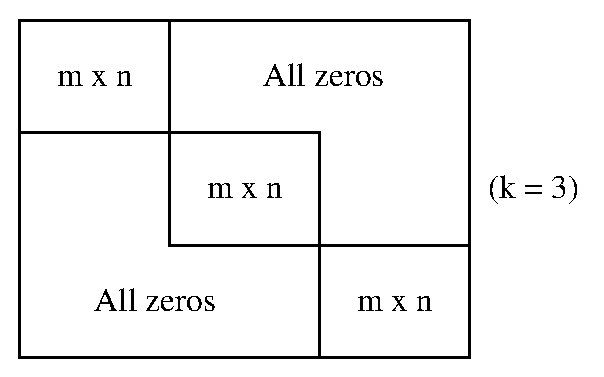
\epsfig{file=figure2.eps,width=4.0in}
\end{center}
\vspace{-0.2in}
\caption{Illustrating why $f(km,kn) \geq f(m,n)$}
\label{fig2}
\end{figure}

More generally, we can show that
\begin{equation*}
f(m_1+\cdots+m_k, n_1+\cdots+n_k) \geq min[f(m_1,n_1),f(m_2,n_2),\cdots,f(m_k,n_k)]
\end{equation*}
The inequality $f(k,m) \cdot f(m,n) \leq f(k,n)$ can be rewritten as
\begin{equation*}
f(m,n) \leq f(k,n) / f(k,m).
\end{equation*}
Setting $k = 1$, we obtain
\begin{equation*}
f(m,n) \leq \sqrt{n/m},
\end{equation*}
as we found earlier (with equality if and only if m divides n).

Setting k = 2, we find that
\begin{equation*}
f(m,n) \leq f(2,n) / f(2,m).
\end{equation*}
We now know that if $j$ is even, then $f(2,j) = \sqrt{j/2}$, whereas if j is
odd, then $f(2,j) = \sqrt{(4j-3)/8}$.  If $m$ is even and $n$ is odd, we
obtain
\begin{equation*}
f(m,n) \leq f(2,n) / f(2,m) = \sqrt{(4n-3)/(4m)}.
\end{equation*}
which is a better bound than $\sqrt{n/m}$ except when $m = 2$.  Thus, for
example, if $n = m+1$, we have $f(m,m+1) \leq \sqrt{(4m+1)/(4m)}$.  So, for
$m = 4$, $n = 5$, the new bound gives $f(4,5) \leq \sqrt{17/16} \approx
1.0307764$, whereas the earlier bound gave $f(4,5) < \sqrt{5/4} \approx
1.1180340$.

\section*{When does $f(m,n) = f(2,n)/f(2,m)$?}
\addcontentsline{toc}{section}{When does $f(m,n) = f(2,n)/f(2,m)$?}

For $m$ even and $n$ odd, we shall investigate when equality occurs in
\begin{equation*}
f(m,n) \leq \sqrt{(4n-3)/(4m)}
\end{equation*}
For $m = 2$, it is trivially true that $f(2,n) = f(2,n) / f(2/2)$, so we will
only consider $m \geq 4$.  When is the largest square in an $m$-cube also one
of the largest squares in the $n$-cube, with the $m$-cube in the $n$-cube?  We
shall use normalization appropriate for a unit $n$-cube.  Then,
\begin{equation*}
\sum_{i=1}^{m/2}   \vec{v}_i = \vec{w}_1 ~~~\text{and}~~
\sum_{i=m/2+1}^{m} \vec{v}_i = \vec{w}_2
\end{equation*}
where $\vec{w}_1$ is something like (3/4, 3/4, 0, 0, 1) and $\vec{w}_2$ is
something like (1/4, -1/4, 1, 1, 0).

That is, for $i = 1,2$, $j = 1$ to $n$, $w_{ij} = 0, \pm1, \pm1/4, \pm3/4$,
with $\pm3/4$ and $\pm1/4$ appearing exactly twice, etc. so that $|w_{1i}| +
|w_{2i}| = 1$ for all $i = 1$ to $n$.  Thus,
\begin{equation*}
\sum_{i=1}^{m/2}   v_{ij} ~~+
\sum_{i=m/2+1}^{m} v_{ij} ~=~ 1 ~~~\text{for all}~~ j = 1, 2, \cdots, n
\end{equation*}
But $|\sum_{i=1}^{m/2}   v_{ij}| \leq \sum_{i=1}^{m/2}   |v_{ij}|$
and $|\sum_{i=m/2+1}^{m} v_{ij}| \leq \sum_{i=m/2+1}^{m} |v_{ij}|$
and $\sum_{i=1}^{m} |v_{ij}| \leq 1$,
so
\begin{equation*}
\sum_{i=1}^{m} |v_{ij}| = 1.
\end{equation*}
Now, $\sum_{i=1}^{m/2}   v_{ij} = w_{1j}$
and  $\sum_{i=m/2+1}^{m} v_{ij} = w_{2j}$
implies
\begin{itemize}
\item[]{If $w_{1j} \geq 0$ for some $j$, then $v_{ij} \geq 0$ for all $i \leq m/2$}
\item[]{If $w_{1j} \leq 0$ for some $j$, then $v_{ij} \leq 0$ for all $i \leq m/2$}
\end{itemize}
\label{refpage19}
Similarly for $w_{2j}$ and $i > m/2$.

However, the $\vec{v}_i$ are all orthogonal, so that if some $v_{ij} \neq 0$
for some $i \leq m/2$, then all other $v_{ij} = 0$ for the same j and other $i
\leq m/2$.  Similarly for $i > m/2$.

Therefore, for every $i \leq m/2$, if one of the $v_{ij}$ is equal to
\label{refpage20}
$w_{1j}$, then for all other $j$, $v_{ij} = 0$.  Similarly for $i > m/2$ and
$w_{2j}$.

But the $\vec{v}_i$ all have equal squared length.  The squared lengths cannot
be equal unless for each $i \leq m/2$ there is a $v_{ij} = \pm 3/4$ and for
each $i > m/2$ there is a $v_{ij} = \pm 1/4$, or vice versa.  There are only
two $v_{ij} = \pm 3/4$ and only two $v_{ij} = \pm 1/4$, so $m$ can only be 4.
The only possibility is that for each $i \leq m/2$, the $v_{ij}$ consist of
one $\pm 3/4$ and $(n-3)/4$ $\pm 1$'s, and the rest zeros, and for each $i >
m/2$ the $v_{ij}$ consist of one $\pm 1/4$ and $(n-1)/4$ $\pm 1$'s, and the
rest zeros (or vice versa).

However, $(n-3)/4$ and $(n-1)/4$ cannot both be integers, a contradiction.
This proves that for $m$ even and $\geq 4$, and $n$ odd, $f(m,n)$ is strictly
less than $\sqrt{(4n-3)/(4m)}$.

\section*{General Infinitesimal Rotations}
\addcontentsline{toc}{section}{General Infinitesimal Rotations}

We now consider a general method of finding the largest $m$-cube(s)
in an $n$-cube, by applying an arbitrary infinitesimal rotation to
the $\vec{v}_i$. This technique reduces the problem to a system of polynomial
equations and inequalities. We will illustrate this method for $m = 3$, $n =
4$, but it can be applied to any $m$ and $n$.

In 4-dimensional space, an infinitesimal rotation matrix has the form
\begin{equation}
\label{eqn1}
1 + E =
\begin{bmatrix}
~1~     & ~~e_{12} & ~~e_{13} & ~e_{14}~ \\
-e_{12} &  ~1~     & ~~e_{23} & ~e_{24}~ \\
-e_{13} &  -e_{23} &  ~1~     & ~e_{34}~ \\
-e_{14} &  -e_{24} &  -e_{34} &  1~~
\end{bmatrix}
\end{equation}
Let the matrix $1 + E$ in (\ref{eqn1}) be multiplied by the transpose of the $V$
matrix:
\begin{equation*}
V =
\begin{bmatrix}
A & B & C & D \\
F & G & H & J \\
K & L & M & P
\end{bmatrix}
\end{equation*}
\begin{equation*}
V^\top =
\begin{bmatrix}
A & F & K \\
B & G & L \\
C & H & M \\
D & J & P
\end{bmatrix}
\end{equation*}
Then
\begin{align*}
(1 + E) \, & V^\top = \\
& \left[
\begin{array}{rrr}
 A + B \, e_{12} + C \, e_{13} + D \, e_{14} &
\cdots                                       &
 K + L \, e_{12} + M \, e_{13} + P \, e_{14} \\
-A \, e_{12} + B + C \, e_{13} + D \, e_{24} &
\cdots                                       &
-K \, e_{12} + L + M \, e_{13} + P \, e_{24} \\
-A \, e_{13} - B \, e_{23} + C + D \, e_{34} &
\cdots                                       &
-K \, e_{13} - L \, e_{23} + M + P \, e_{34} \\
-A \, e_{14} - B \, e_{24} - C \, e_{34} + D &
\cdots                                       &
-K \, e_{14} - L \, e_{24} - M \, e_{34} + P
\end{array}
\right]
\end{align*}
which is a 4x3 matrix.

If we take absolute values and assume for now that the matrix $V$ contains no
zeros, we find that the infinitesimal rotation converts $R_1$ to $R_1'$, $R_2$
to $R_2'$, etc., where
\begin{alignat*}{4}
R_1' - R_1 & = a(B \, e_{12} + &&\:C \, e_{13} + D \, e_{14}&&) &&+ f (\cdots \\
R_2' - R_2 & = b(              &&~\cdots                    &&) &&+ ~\cdots \\
R_3' - R_3 & = c(              &&~\cdots                    &&) &&+ ~\cdots \\
R_4' - R_4 & = d(              &&~\cdots                    &&) &&+ ~\cdots
\end{alignat*}
where $a$ = sign($A$), $b$ = sign($B$), etc.; that is, $a = 1$ if $A$ is
positive and $a = -1$ if $A$ is negative, etc.  This may be written as
\begin{equation*}
\begin{bmatrix}
R_1' - R_1 \\
R_2' - R_2 \\
R_3' - R_3 \\
R_4' - R_4 
\end{bmatrix}
= T
\begin{bmatrix}
e_{12} \\
e_{13} \\
e_{14} \\
e_{23} \\
e_{24} \\
e_{34} 
\end{bmatrix}
\end{equation*}
where $T$ is the following 4x6 matrix:
\begin{equation*}
\tiny
\begin{bmatrix}
~~aB+fG+kL & ~~aC+fH+kM & ~~aD+fJ+kP &      0     &      0     &      0     \\
 -bA-gF-lK &      0     &      0     & ~~bC+gH+lM & ~~bD+gJ+lP &      0     \\
     0     &  -cA-hF-mK &      0     &  -cB-hG-mL &      0     & ~~cD+hJ+mP \\
     0     &      0     &  -dA-jF-pK &      0     &  -dB-jG-pL &  -dC-jH-pM
\end{bmatrix}
\normalsize
\label{refpage10}
\end{equation*}
Now, suppose that the original $V$ matrix has only one maximal column, the
first.  Then we can decrease R if there is some choice of the $e_{ij}$'s for
which $R_1' - R_1 < 0$.  This is possible provided that $T_{11}$, $T_{12}$,
and $T_{13}$ are not all zero.  In general, if $V$ has any number of maximal
columns, we can decrease $R$ if the matrix $T_{mod}$ consisting of the
corresponding rows of $T$ has maximum rank.  So, to find all possible cube
orientations which might be locally optimal, we need to determine when
$T_{mod}$ has less than maximum rank.

The procedure is slightly more complicated if $V$ contains zeros in any of is
maximal columns.  For instance, if $A = 0$, then we have to deal with absolute
values such as $|B\,e_{12}+C\,e_{13}+D\,e_{14}|$ in the expression for $R_1' -
R_1$.  We can proceed as follows:  If $A = 0$, then we consider the inequality
\begin{equation*}
B\,e_{12}+C\,e_{13}+D\,e_{14} > 0
\end{equation*}
and replace $a$ by 1 in the equation for $R_1' - R_1$.

Including this equation with the others corresponds to adding another row to
$T_{mod}$
\begin{equation*}
\begin{bmatrix}
B & C & D & 0 & 0 & 0
\end{bmatrix}
\end{equation*}
Then, if we cannot make $T_{mod}$ applied to (or multiplied by)
\begin{equation*}
\begin{bmatrix}
e_{12} \\
e_{13} \\
e_{14} \\
e_{23} \\
e_{24} \\
e_{34} 
\end{bmatrix}
\end{equation*}
equal to anything we like, it much be that $T_{mod}$ has less than maximum
rank.

We may also consider the effects of $|B\,e_{12}+C\,e_{13}+D\,e_{14}| = 0$ and
$|B\,e_{12}+C\,e_{13}+D\,e_{14}| < 0$.  But these lead to matrices of the same
rank and need not be treated separately.

We have been assuming that $T_{mod}$ has no more rows than it has
columns. If this condition is not satisfied, then, instead of using a
$T_{mod}$
matrix, we need to solve a system of equations; for instance, we could be
considering the case in which $V$ is snug-fitting ($R = R_1 = R_2 = R_3 = R_4$)
and the matrix elements $A$, $G$, and $M$ are zero, in addition to the
orthonormality of the rows of $V$. This leads to 9 polynomial equations in 9
unknowns. Not surprisingly, we have not been able to solve these
equations and find out whether we can obtain a larger cube in a tesseract
than the one we have already discussed. However, there are algorithms
for doing this, which are described in \cite{cox1992}.

Now consider a cube in a tesseract with $R = R_1 > R_2, R_3, R_4$, with
no zeros in the first column of $V$. For possible optimality, $T_{mod}$ must
have rank zero, where
\begin{equation*}
T_{mod} =
\begin{bmatrix}
aB\!\!+\!\!fG\!\!+\!\!kL & aC\!\!+\!\!fH\!\!+\!\!kM & aD\!\!+\!\!fJ\!\!+\!\!kP & 0 & 0 & 0
\end{bmatrix}
\end{equation*}
This implies that the first three elements of $T_{mod}$ are zero.  Thus,
\begin{equation*}
a\,(B,C,D) + f\,(G,H,J) + k\,(L,M,P) = (0,0,0)
\end{equation*}
This means that $\pm \vec{v}_1 \pm \vec{v}_2 \pm \vec{v}_3$ contains 3 zero
components for some combination of signs.  However, it is impossible for $\pm
\vec{v}_1 \pm \vec{v}_2 \pm \vec{v}_3$ to contain even one or more zero
components for any combination of signs, by a generalization of Phil DeVicci's
Theorem.  For if it does, then a main diagonal of the cube fits into a unit
cube parallel to one of the hyperfaces of the unit tesseract.  Therefore, the
cube has a side less than or equal to 1 and is not optimal.  Phillip DeVicci
proved that for $m = 2$, $n = 3$, $\vec{v}_1 + \vec{v}_2$ could not have any
zero components.

Next, let us consider $R = R_1 = R_2 > R_3, R_4$ with no zeros in the first 2
columns of $V$.  Then $T_{mod}$ is
\begin{equation*}
\footnotesize
\begin{bmatrix}
 aB+fG+kL &  aC+fH+kM &  aD+fJ+kP &     0     &     0     &     0     \\
-bA-gF-lK &     0     &     0     &  bC+gH+lM &  bD+gJ+lP &     0 
\end{bmatrix}
\normalsize
\end{equation*}
has rank 1 or less, so some linear combination of the two rows of $T_{mod}$ is
zero. This is obviously impossible by GPT (Generalization of Phil's
Theorem). In fact, the same thing happens when there are 3 maximal
columns containing no zeros. An optimal $V$ matrix with no zeros must be
snug-fitting, as we proved previously.

Next, we consider the case in which only the first column is
maximal, with $A = 0$ and no other zeros in this column. Thus we have
\begin{equation*}
T_{mod} =
\begin{bmatrix}
 B\!+\!fG\!+\!kL &  C\!+\!fH\!+\!kM &  D\!+\!fJ\!+\!kP & 0 & 0 & 0 \\
 B               &  C               &  D               & 0 & 0 & 0
\end{bmatrix}
\end{equation*}
or, more simply,
\begin{equation*}
\begin{bmatrix}
 fG\!+\!kL &  fH\!+\!kM &  fJ\!+\!kP & 0 & 0 & 0 \\
 B         &  C         &  D             & 0 & 0 & 0
\end{bmatrix}
\end{equation*}
must have rank 1 or less.  This implies that $(B,C,D)$ and $f(G,H,J)+k(L,M,P)$
are parallel.

Recall that in this case
\begin{equation*}
V = 
\begin{bmatrix}
0 & B & C & D \\
F & G & H & J \\
K & L & M & P
\end{bmatrix}
\end{equation*}
Since $\vec{v}_1 \bot \vec{v}_2$, $(B,C,D) \bot (G,H,J)$ and $(B,C,D) \bot
\label{refpage26}
(L,M,P)$.  Also, $f$ and $k$ are each 1 and -1.  So $(B,C,D) \bot f(G,H,J) +
k(L,M,P)$.  But the only way that two vectors can be both parallel and
perpendicular is if one or both are the zero vector.  If $(B,C,D)$ were zero,
then $|\vec{v}_1|$ would be zero, which is impossible.  Thus, $(G,H,J) \pm
(L,M,P)$ must be zero, which implies that $\vec{v}_2 \pm \vec{v}_3$ must
contain three zeros.  But $\vec{v}_2 \pm \vec{v}_3$ cannot contain two or more
zeros by GPT.  For if $s$ is the side of the cube in the unit tesseract, then
$\vec{v}_2 \pm \vec{v}_3$ has length $s\sqrt{2}$.  This must fit parallel to
one of the coordinate planes inside the tesseract, and cannot be longer than
the diagonal of a square with side length 1, so $s\sqrt{2} \leq \sqrt{2}$.
Thus, $s \leq 1$ and the cube cannot be optimal.

Similar proofs can be used to show that $A = 0$ is also impossible if
\label{refpage6}
the first 2 or the first 3 columns are the only maximal ones and do not
contain any additional zeros. Again we find that only the snug-fitting
case can be optimal.

Similar proofs also apply to 2 zeros either in the same row or the
same column of $V$. That is, if $A$ and $B$ are the only zero elements in the
first 2 columns, and only these columns are maximal, then $V$ cannot be
optimal, nor can it be optimal if there is a third maximal column
containing no zeros; also, if $A$ and $F$ are the only zero elements in the
first column, and only this column is maximal, then $V$ cannot be optimal, nor
can it be optimal if there are one or two other maximal columns
containing no zeros.

However, if the 2 zeros are in neither the same row nor the same
column, then the problem is more difficult. If $A$ and $G$ are zero and are the
only zero elements in the first two columns, and the first two columns
are the only maximal columns, then we can prove that $V$ is not optimal,
and because of the difficulty of the proof, we shall describe it here in
detail. $T_{mod}$ is shown below:
\begin{equation*}
\begin{bmatrix}
 kL & fH+kM & fJ+kP &  0    &  0    & 0~ \\
  B &  C    &  D    &  0    &  0    & 0~ \\
-lK &  0    &  0    & bC+lM & bD+lP & 0~ \\
 -F &  0    &  0    &  H    &  J    & 0~
\end{bmatrix}
\end{equation*}
Assume that some linear combination of the rows of $T_{mod}$ is zero, with
coefficients $a_1$, $a_2$, $a_3$, $a_4$, respectively.

If only $a_1$ is nonzero, then $f(H,J) + k(M,P) = (0,0)$, so $V$ cannot be
optimal by GPT.  Similarly if only $a_3$ is nonzero.

If only $a_2$ is nonzero, then $B$, $C$, and $D$ are all zero, which is
impossible.  Similarly if only $a_4$ is nonzero.

If only $a_1$ and $a_2$ are nonzero, then $a_1 [f(G,H,J)+k(L,M,P)] + a_2
(B,C,D) = 0$. Thus,
\begin{equation}
\label{eqn2}
f(G,H,J) + k(L,M,P) = -(a_2/a_1)(B,C,D).
\end{equation}
But $f(G,H,J)+k(L,M,P) \bot (B,C,D)$.

Taking the dot product of both sides of (\ref{eqn2}) with $(B,C,D)$ yields $B
= C = D = 0$, which is impossible.

If only $a_1$ and $a_3$ are nonzero, then $f(H,J)+k(M,P) = 0$ - non-optimal by
GPT.

If only $a_1$ and $a_4$ are nonzero, then $H$ and $J$ are 0 - non-optimal.

If only $a_2$ and $a_3$ are nonzero, then $C$ and $D$ are 0 - non-optimal.

If only $a_2$ and $a_4$ are nonzero, then $C$ and $D$ are 0 - non-optimal.

If only $a_3$ and $a_4$ are nonzero, this is similar to $a_1$ and $a_2$
\label{refpage7}
nonzero.

If exactly 3 of the $a_i$ are nonzero, a similar situation occurs.  Thus, we
now assume that all four $a_i$ are nonzero.

We have
$a_1[f(H,J)+k(M,P)] + a_2(C,D) = 0$ and
$a_3[b(C,D)+l(M,P)] + a_4(H,J) = 0$.

Let $\vec{u} = (C,D)$, $\vec{v} = (H,J)$, and $\vec{w} = (M,P)$.  Then
$a_1(f \vec{v} + k \vec{w}) + a_2 \vec{u} = 0$, and
$a_3(b \vec{u} + l \vec{w}) + a_4 \vec{v} = 0$.  Neither $\vec{u}$ nor
$\vec{v}$ is zero as this would make $V$ non-optimal.  Also, if $\vec{w} = 0$
then $\vec{u}$ and $\vec{v}$ are parallel.  But $\vec{u}$ and $\vec{v}$ are
also perpendicular, because $A = G = 0$, and nonzero which is a contradiction.
So $\vec{w}$ is also nonzero.  Thus,
\begin{align*}
\vec{u} & = C_1 (f\,\vec{v} + k\,\vec{w}) \\
\vec{v} & = C_2 (b\,\vec{u} + l\,\vec{w}),
\end{align*}
with $C_1$ and $C_2$ nonzero.  Substituting each of the last 2 equations into
the other yields
\begin{align}
\label{eqn3}
(1 - C_1\,C_2\,f\,b)\,\vec{u} & = C_1 (f\,l\,C_2 + k)\,\vec{w} \\
\label{eqn4}
(1 - C_1\,C_2\,f\,b)\,\vec{v} & = C_2 (b\,k\,C_1 + l)\,\vec{w}
\end{align}
If $f l C_2+k = 0$, then $C_1 C_2 f b = 1$.  Since $f$, $b$, and $l$ are
$\pm 1$, we have $C_1 C_2 = f $, and $C_2 = -k f l$, so $C_1 = -k b l$.
Thus $\vec{u} = \pm \vec{v} \pm \vec{w}$, so $V$ is non-optimal by GPT.

Similarly, if $b k C_1 + l = 0$, and $C_1 C_2 f b = 1$, so $C_1 C_2 = f b$,
and $C_1 = -l b k$, $C_2 = -l f k$, so $\vec{v} = \pm \vec{u} \pm \vec{w}$, so
$V$ is non-optimal.  Thus the right-hand sides of (\ref{eqn3}) and
(\ref{eqn4}) are nonzero.  This shows that $\vec{u}$ and $\vec{w}$ are
parallel, and so are $\vec{v}$ and $\vec{w}$.  Since $\vec{u}$, $\vec{v}$, and
$\vec{w}$ are all nonzero, it follows that $\vec{u}$ and $\vec{v}$ are
parallel.  Since $\vec{u}$ and $\vec{v}$ are also perpendicular to each other,
we have a contradiction, which proves that $a_1$ through $a_4$ are all zero
and thus $T_{mod}$ cannot have less than rank 4 in this case, so $V$ is
non-optimal.

If $A$ and $G$ are zero and are the only zero elements in the first three
columns, which are the only maximal columns, then it is trivial to show
that as must be zero. Then this case reduces to the previous case. Thus
we have shown that if $A$ = $G$ = 0 and the first 2 columns (at least) are
maximal and $A$ and $G$ are the only zeros in the maximal columns, then $V$
must be snug-fitting to be optimal.

To illustrate an even more difficult case, consider the case of $A = G = M =
0$, with $R = R_1 = R_2 = R_3 > R_4$.  Thus $V$ looks like this:
\begin{equation*}
V =
\begin{bmatrix}
0 & B & C & D \\
F & 0 & H & J \\
K & L & 0 & P \\
\end{bmatrix}
\end{equation*}
and
\begin{equation*}
T_{mod} =
\begin{bmatrix}
 kL &  fH & fJ+kP &   0 &  0    &  0    \\
-lK &   0 &  0    &  bC & bD+lP &  0    \\
  0 & -hF &  0    & -cB &  0    & cD+hJ \\
  B &   C &  D    &   0 &  0    &  0    \\
 -F &   0 &  0    &   H &  J    &  0    \\
  0 &  -K &  0    &  -L &  0    &  P
\end{bmatrix}
\end{equation*}
Then we will have 9 equations in 9 unknowns:  6 equations for orthonormality:
$CH + DJ = 0$, $B^2 + C^2 + D^2 = 1$, etc.; also, $R_1 = R_2$, and $R_2 = R_3$
and finally det($T_{mod}$) = 0.  With no loss of generality, $D$, $J$, and $P$
may be assumed positive (we shall show later that a maximal cube in a
tesseract cannot have more than 3 zeros in its $V$ matrix).  Also, we may
assume then $C > 0$, which makes $H < 0$; and assume $L > 0$, which makes $B <
0$, and assume $F > 0$, so that $K < 0$.  Thus in $T_{mod}$, $k = -1$, $f =
1$, $b = -1$, etc.; there is only one set of signs to consider.  But we still
have a horrible set of 9 polynomial equations in 9 unknowns.

In general, we always get a system of polynomial equations with
integer coefficients (including the setting of sub-determinants to zero),
together with inequalities such as $C > 0$, $H < 0$, and $C - H > 0 + J + P$.

The snug-fitting case with exactly two zeros in the same row, and
\label{refpage21}
all other elements non-zero, can be shown to be non-optimal, but we omit
the proof.

We have seen that an optimal $V$ matrix with no zeros must be snug-fitting.
\label{refpage2start}
We shall derive equations for one of these sub-cases. There are
more than one sub-case because each element of $V$ may be positive or
negative. Many of these sub-cases can be eliminated as equivalent to
others, because we may change all the signs in any row or column, or
permute rows or columns. Other sub-cases can be eliminated by the
constraint that the rows of $V$ are orthogonal. Still other sub-cases can be
shown to be non-optimal by Theorem 2 in the section on plane rotations,
together with GPT. Here is an example:
\begin{equation*}
\begin{bmatrix}
A & B & C & D \\
F & G & H & J \\
K & L & M & P
\end{bmatrix}
=
\begin{bmatrix}
+ & + & + & + \\
+ & + & - & - \\
+ & - & + & -
\end{bmatrix}
\end{equation*}
We use the normalization here in which all column-sums are equal to 1.  Thus a
cube cannot be maximal unless $A^2 + B^2 + C^2 + D^2$ (or $F^2 + G^2 + H^2 +
J^2$, etc. -- they are all equal) is greater than 1.  If fact, it must be at
least $1.007434...^2$.

By GPT, no matrix element my be $\pm 1/2$.  Then, by Theorem 2 applied to
\label{refpage1start}
columns 1 and 2, either $|K|$ and $|L|$ are $> 1/2$ and $|A| + |F|$ and $|B| +
|G| < 1/2$, or $|K|$ and $|L|$ are $< 1/2$ and $|A| + |F|$ and $|B| + |G| >
1/2$.  Next we apply the theorems to columns 3 and 4, obtaining an analogous
result.  We can eliminate two of the ``sub-sub-cases'' because they lead to one
or more row vectors with a length less than 1. Then we can apply Theorem 2 to
columns 1 and 3, and then ~o 2 and 4, and similar arguments will eliminate
\label{refpage2end}
the entire sub-case.

Now let us consider $T_{mod}$, which, with no non-maximal columns and
no zeros, is identical with the 4x6 matrix $T$.

For an optimal cube, $T$ must have rank less than 4. This is equivalent
to the property that all 4x4 sub-determinants are zero; but it is easier in
this case to consider linear combinations of the rows of $T$, with
coefficients $a1$, $a2$, $a3$, and $a4$, and set the linear combinations
equal to zero.

From GPT, no element of $T$ such as $aB+fG+kL$ can be equal to zero.

In
\begin{equation*}
V =
\begin{bmatrix}
A & B & C & D \\
F & G & H & J \\
K & L & M & P
\end{bmatrix}
\end{equation*}
let us assume that $J$, $M$, and $P$ are negative, with all the other elements
\label{refpage8}
of $V$ positive.  We now set
\label{refpage9}
\begin{alignat*}{11}
a_1 &(B&&+G&&+L&&) &&+ a_2 &&(-&&A&&-F&&-K&&) &&= 0 \\
a_1 &(C&&+H&&+M&&) &&+ a_3 &&(-&&A&&-F&&+K&&) &&= 0 \\
a_1 &(D&&+J&&+P&&) &&+ a_4 &&(-&&A&&+F&&+K&&) &&= 0 \\
a_2 &(C&&+H&&+M&&) &&+ a_3 &&(-&&B&&-G&&+L&&) &&= 0 \\
a_2 &(D&&+J&&+P&&) &&+ a_4 &&(-&&B&&+G&&+L&&) &&= 0 \\
a_3 &(D&&+J&&+P&&) &&+ a_4 &&(-&&C&&+H&&+M&&) &&= 0
\end{alignat*}
However, the cube is snug-fitting, so that $A\!+\!F\!+\!K = B\!+\!G\!+\!L
= C\!+\!H\!-\!M = D\!-\!J\!-\!P$.
We may normalize $V$ so that these sums and differences are all equal to 1.
We find that $a_1 = a_2$,so the equations simplify. Note that if anyone
of $a_1$, $a_2$, $a_3$, and $a_4$ is zero, then they are all zero. So we may
assume that they are all nonzero.

Also, $-\!A\!-\!F\!+\!K = -1\!+\!2K$, etc.
\begin{alignat*}{6}
a_1/a_3 &=  (A+&&F-&&K  &&)/  (C &&+&&\!\!\!H+M)         \\
        &= (1~-&&~2K&&)/&&(1\:+\:&&2M&&)           \\
a_1/a_4 &= (1~-&&~2A&&)/&&(1\:-\:&&2D&&)           \\
a_2/a_3 &= (1~-&&~2L&&)/&&(1\:+\:&&2M&&) = a_1/a_3 \\
a_2/a_4 &= (1~-&&~2B&&)/&&(1\:-\:&&2D&&) = a_1/a_4 \\
a_3/a_4 &= (1~-&&~2H&&)/&&(1\:+\:&&2J&&)
\end{alignat*}
From these equations we see that $A = B$ and $K = L$.  In fact, since $R_1 =
\label{refpage11}
R_2$, the first 2 columns of $V$ are identical.  Thus we have only 9 unknowns
instead of 12.  In addition, we get another equation, since
\begin{equation*}
(a_1/a_3)(a_3/a_4)(a_4/a_1) = 1,
\end{equation*}
we obtain $(1\!+\!2M)(1\!+\!2J)(1\!-\!2A) = (1\!-\!2K)(1\!-\!2H)(1\!-\!2D)$.
\label{refpage1end}
We end up with 9 equations in 9 unknowns.

\section*{Zeros in the $V$ matrix for $m = 3$, $n = 4$}
\addcontentsline{toc}{section}{Zeros in the $V$ matrix for $m = 3$, $n = 4$}

Here we show that there cannot be more than 3 zeros in the $V$ matrix
for a maximal cube in a tesseract, and we prove some other restrictions
as well, which are necessary for optimality.

We previously found that if $V$ contains either 0, 1, or 2 zeros in its
maximal columns, and is optimal, then the cube must be snug-fitting.

If there are 3 zeros all in different rows and different columns, then
the cube is either snug-fitting or there are 3 maximal columns -- the
columns containing the zeros.

If there are 3 zeros in one column, the cube is not optimal. The same
applies to 3 zeros in one row. If there are 3 zeros in a triangle:
\begin{equation*}
\begin{array}{cccc}
X & X & 0 & 0 \\
X & X & X & 0 \\
X & X & X & X
\end{array}
\end{equation*}
where the $X$'S may be zero or non-zero, the cube must be snug-fitting.
This is our candidate for optimality. There cannot be any additional zeros.

There are 2 other cases to consider with 3 zeros. One is
\begin{equation*}
\label{refpage5}
\begin{array}{cccc}
0 & X & X & X \\
0 & X & X & X \\
X & 0 & X & X
\end{array}
\end{equation*}
(case 1) and the other is
\begin{equation*}
\begin{array}{cccc}
0 & 0 & X & X \\
X & X & 0 & X \\
X & X & X & X
\end{array}
\end{equation*}
(case 2).

In both cases above, the $X$'s may be zero or nonzero.  In case 1, $V$ can be
parameterized as follows:
\begin{equation*}
\left[
\begin{array}{ccrr}
   0      & sin\beta & -cos\beta ~sin\gamma & -cos\beta ~cos\gamma \\
   0      & cos\beta &  sin\beta ~sin\gamma &  sin\beta ~cos\gamma \\
cos\alpha &    0     & -sin\alpha~cos\gamma &  sin\alpha~sin\gamma \\
\end{array}
\right]
\end{equation*}
We see that $R_2 = |sin\beta| + |cos\beta|$, which is $\geq 1$ for all
$\beta$, so that such a cube cannot be optimal.

Finally, in case 2, for $\vec{v}_1 \bot \vec{v}_2$, either $v_{14}$ or
$v_{24}$ (or both) must be zero.  If $v_{14} = 0$, we have a row of 3 zeros,
so this is not optimal.  If $v_{24} = 0$, we may parameterize $V$ as follows:
\begin{equation*}
\left[
\begin{array}{cccc}
   0      &    0     &  sin\alpha           &  cos\alpha           \\
sin\beta  & cos\beta &           0          &           0          \\
cos\alpha &    0     & -sin\alpha~cos\gamma &  sin\alpha~sin\gamma \\
\end{array}
\right]
\end{equation*}
We introduce primed angles with $0 \leq \alpha',\beta',\gamma' \leq 90^o$.
Then
\begin{alignat*}{2}
R_1 &= sin\beta'  &&+ cos\gamma'~cos\beta'  \\
R_2 &= cos\beta'  &&+ cos\gamma'~sin\beta'  \\
R_3 &= sin\alpha' &&+ sin\gamma'~cos\alpha' \\
R_4 &= cos\alpha' &&+ sin\gamma'~sin\alpha'
\end{alignat*}
Assume first that $0^o \leq \alpha',\beta',\gamma' < 90^o$.  If there is only
one maximal column, we may increase or decrease $\gamma$ to decrease $R$.

If columns 1 and 2, or 3 and 4, are the only maximal columns, we may change
$\gamma$ to decrease both maximal column-sums.

If columns 1 and 3, or 1 and 4, or 2 and 3, or 2 and 4 are the maximal
columns, we may change $\alpha$ and $\beta$ slightly so that on column-sum
decreases and the other is unchanged.

If columns 1, 2, and 3, or 1, 2, and 4 are maximal, then we change $\alpha$
slightly. If columns 1, 3, and 4, or 2, 3, and 4 are maximal, we change
$\beta$ slightly.

If $\alpha'$ or $\beta'$ are $0^o$ or $90^o$, then $R \geq 1$.

If $\gamma'$ is $0^o$ or $90^o$, then one of the column-sums will be
$sin\alpha' + cos\alpha'$ or $sin\beta' + cos\beta'$, so $R \geq 1$.

Thus an optimal cube with this form must be snug-fitting, with $0^o <
\alpha',\beta',\gamma' < 90^o$.  By doing some simple algebra we find that
$\alpha'$, $\beta'$, and $\gamma'$ are all $45^o$, so that $R = 1/2 +
\sqrt{2}/2 > 1$, so that even this is not optimal.

The above also shows that for $m = 3$, $n = 4$, $V$ may not have 4 or more
zeros.  Thus the only possibilities are those shown below where the $X$'s
\label{refpage23}
represent nonzero matrix elements:
\begin{equation*}
\myarrset
\begin{array}{cccccccccccccccccccccccc}
X & X & X & X & ~~~ & 0 & X & X & X & ~~~ & 0 & X & X & X & ~~~ & 0 & X & X & X & ~~~ & X & X & 0 & 0 \\
X & X & X & X & ~~~ & X & X & X & X & ~~~ & 0 & X & X & X & ~~~ & X & 0 & X & X & ~~~ & X & X & X & 0 \\
X & X & X & X & ~~~ & X & X & X & X & ~~~ & X & X & X & X & ~~~ & X & X & X & X & ~~~ & X & X & X & X
\end{array}
\end{equation*}
which must be snug-fitting to be optimal and
\begin{equation*}
\myarrset
\begin{array}{cccc}
0 & X & X & X \\
X & 0 & X & X \\
X & X & 0 & X
\end{array}
\end{equation*}
for which at least the first three columns must be maximal for possible
optimality.  Notice that we have eliminated almost all case that are not
snug-fitting!

\section*{Lagrange Multipliers (again)}
\addcontentsline{toc}{section}{Lagrange Multipliers (again)}

For general $m$ and $n$, an alternative technique to the method of
infinitesimal rotations is Lagrange multipliers.  For instance, consider
\begin{equation*}
\begin{bmatrix}
A & B & C & D \\
F & G & H & J \\
K & L & M & P
\end{bmatrix}
\end{equation*}
with columns 1, 2, and 3 maximal, and $A = G = M = 0$.  Then with no loss of
generality we may assume that $D$, $J$, $P$, $C$, $L$, and $F$ are positive,
and that $B$, $H$, and $K$ are negative.

We want to maximize $A^2+B^2+C^2+D^2$, with $A^2+B^2+C^2+D^2-F^2-G^2-H^2-J^2
= 0$, $A^2+B^2+C^2+D^2-K^2-L^2-M^2-P^2 = 0$, $AF+BG+CH+DJ= 0$, etc.;
also, $|A|+|F|+|K| = = 1$ etc.
so that $F-K = 1$, $L-B = 1$, and $C-H < 1$, and $D+J+P < 1$. However, we
may eliminate $A$, $G$, and $M$ from the problem entirely, since they are all
zero. Thus we want to maximize $B^2+C^2+D^2$, etc. Let the Lagrange
multipliers be $\lambda_1$, $\lambda_2$, etc. We want to apply the constrained
2nd derivative test in \cite{fleming1965}, and the diagonal elements of the
matrix of 2nd partial derivatives include $2(1 + \lambda_1 + \lambda_2)$
(3 times, for $B$, $C$, and $D$), $-2\lambda_1$ (3 times), and $-2\lambda_2$
(3 times).  These add up to 2, which is positive, so at
least one diagonal element is positive. So none of the ``points'' which we
get from Lagrange multipliers are maxima. The only possibility is that
the matrix of first partial derivatives of the (equality) constraints with
respect to $B$, $C$, etc., has less than maximum rank; that is, since there are
now 8 equality constraints and 9 variables, all 8 x 8 sub-determinants can
be set to 0 simultaneously. So again we get a system of polynomial
equations with integer coefficients, together with a set of strict
inequalities of a similar form.

The matrix of first partial derivatives is
\begin{equation*}
\left[
\begin{array}{rrrrrrrrr}
2B & 2C & 2D & -2F & -2H & -2J &   0 &   0 &   0 \\
2B & 2C & 2D &   0 &   0 &   0 & -2K & -2L & -2P \\
 0 &  H &  J &   0 &   C &   D &   0 &   0 &   0 \\
 L &  0 &  P &   0 &   0 &   0 &   0 &   B &   D \\
 0 &  0 &  0 &   K &   0 &   P &   F &   0 &   J \\
 0 &  0 &  0 &   K &   0 &   P &   F &   0 &   J \\
 0 &  0 &  0 &   1 &   0 &   0 &  -1 &   0 &   0 \\
-1 &  0 &  0 &   0 &   0 &   0 &   0 &   1 &   0 \\
 0 &  1 &  0 &   0 &  -1 &   0 &   0 &   0 &   0
\end{array}
\right]
\end{equation*}
Instead, we may use the other normalization in which $|A|+|F|+|K| =
|B|+|G|+|L|$, with $A^2+B^2+C^2+D^2 = 1$, etc., and minimize $|A|+|F|+|K|$.
This also leads to the same sorts of polynomial equations and inequalities
with integer coefficients.

\section*{Further Comments and Unsolved Problems}
\addcontentsline{toc}{section}{Further Comments and Unsolved Problems}

We have seen that the problem of the largest m-cube in an n-cube
can be reduced to a finite number of systems of simultaneous polynomial
equations and inequalities with integer coefficients, either by using
Lagrange multipliers or by using our earlier method. In \cite{cox1992} it
is shown how to solve such systems of equations, even with arbitrary
coefficients, using an algorithm which eliminates the variables one by one.
If there are only a finite number of complex solutions, then one could test
each real solution to find which one maximizes the function to be maximized, of
those which satisfy the inequalities. Then one could also prove that the
maximum value is an algebraic number if the coefficients are integral,
rational, or even arbitrary real algebraic numbers. However, this
argument breaks down if there is a continuous infinity of complex
solutions. It would be nice to be able to prove that, even in this case, the
optimal value is algebraic (i.e., that $f(m,n)$ is algebraic for all m, n), and
if it is, there remains the question of whether there is an algorithm which
produces the exact value of $f(m,n)$ (by finding a polynomial equation
which it satisfies, and describing it as, say, the 47th smallest real root
of that equation).

It would not be surprising if we do sometimes get a continuous
infinity of solutions, since if the $V$ matrix has 2 or more non-maximal
columns, these columns could be rotated into each other to produce a
continuous infinity of solutions, all with the same value of $R$.

Many other geometry problems can be put into the form of
optimization problems in which the function to be optimized is a
polynomial function of several variables, with polynomial (equality and
inequality) constraints, all with coefficients that are either integers or,
in some cases, real algebraic numbers. These include the unsolved
problem of finding the largest regular dodecahedron in a regular
icosahedron (and vice versa); it would be interesting to be able to know
immediately that the ratio of the edges or volumes must be an algebraic
number. Even the kissing sphere problem in any number of dimensions can
be reduced to problems of this form. (These problems are discussed in
\cite{croft1991}, \cite{croft1980maximal}. See also
\cite{coxeter1973}, pp.  52-53, where the vertices of the coordinates of
regular dodecahedra and icosahedra are given.)

At this time, we still do not know whether our candidate for the
largest cube in a tesseract is optimal. Perhaps a computer-assisted proof
will finally settle this question, unless there is a more elegant way to
prove it. It would also be interesting to know if the largest m-cube in an
n-cube is snug-fitting for all m and n, as it is for the cases for which we
have solved the problem. Perhaps future work will find additional simple
patterns in $f(m,n)$, as we found for $m = 2$. For instance, one of our general
inequalities was $f(m,n+m)^2 \geq f(m,n)^2 + 1$. It seems entirely possible at
this time that the equal sign always applies. In my opinion, either a proof
or a counterexample would be interesting.

\section*{Prince Rupert's Problem}
\addcontentsline{toc}{section}{Prince Rupert's Problem}

Prince Rupert is discussed in \cite{britannica1964},\cite{schreck1950a},
and Prince Rupert's problem and a generalization of it are discussed in
\cite{schreck1950a},\cite{schreck1950b}.

Prince Rupert (1619-1682) was born in Prague and educated in the
Netherlands. He was also called Rupert of the Rhine or of the Palatinate,
and he was a nephew of King Charles I of Great Britain and Ireland. He was
a royalist cavalry commander in the English civil war. He also dabbled in
scientific experiments and became a member of the Royal Society. Not
only did he have a geometry problem named after him, but he also had an
alloy named after him (still called Prince's metal), and he studied the
properties of quickly cooled drops of glass, known as Rupert drops, in the
laboratory which he had built for himself.

Prince Rupert proposed, but apparently did not solve, the following
problem: ``To perforate a cube in such a way that a second cube of the
same size may pass through the hole'' \cite{schreck1950a}, page 73. Pieter
Nieuwland (1764-1794) not only found that this was possible, but he also
found the size of the largest cube which could pass through such a hole.

Many authors seem to assume, without proof, that this problem is
equivalent to finding the largest square in a cube. The reader may enjoy
investigating this question (the problems do seem to give the same
numerical result for $m = 2$, $n = 3$) for an arbitrary number of dimensions
(i.e., is the problem of finding the largest m-cube in an (m+1)-cube
equivalent to finding the largest (m+1)-cube which can pass through a
``hypercubical'' hole in another (m+1)-cube?). For the most trivial case,
that of passing a line segment through a hole in a square, the square
breaks up into 2 pieces, and for the limiting size, the area of the square
disappears completely.
